% Options for packages loaded elsewhere
\PassOptionsToPackage{unicode}{hyperref}
\PassOptionsToPackage{hyphens}{url}
%
\documentclass[
  14pt,
  ignorenonframetext,
  aspectratio=169,
]{beamer}
\usepackage{pgfpages}
\setbeamertemplate{caption}[numbered]
\setbeamertemplate{caption label separator}{: }
\setbeamercolor{caption name}{fg=normal text.fg}
\beamertemplatenavigationsymbolsempty
% Prevent slide breaks in the middle of a paragraph
\widowpenalties 1 10000
\raggedbottom

\usepackage{amsmath,amssymb}
\usepackage{iftex}
\ifPDFTeX
  \usepackage[T1]{fontenc}
  \usepackage[utf8]{inputenc}
  \usepackage{textcomp} % provide euro and other symbols
\else % if luatex or xetex
  \usepackage{unicode-math}
  \defaultfontfeatures{Scale=MatchLowercase}
  \defaultfontfeatures[\rmfamily]{Ligatures=TeX,Scale=1}
\fi
\usepackage{lmodern}
\ifPDFTeX\else  
    % xetex/luatex font selection
\fi
% Use upquote if available, for straight quotes in verbatim environments
\IfFileExists{upquote.sty}{\usepackage{upquote}}{}
\IfFileExists{microtype.sty}{% use microtype if available
  \usepackage[]{microtype}
  \UseMicrotypeSet[protrusion]{basicmath} % disable protrusion for tt fonts
}{}
\makeatletter
\@ifundefined{KOMAClassName}{% if non-KOMA class
  \IfFileExists{parskip.sty}{%
    \usepackage{parskip}
  }{% else
    \setlength{\parindent}{0pt}
    \setlength{\parskip}{6pt plus 2pt minus 1pt}}
}{% if KOMA class
  \KOMAoptions{parskip=half}}
\makeatother
\usepackage{xcolor}
\newif\ifbibliography
\setlength{\emergencystretch}{3em} % prevent overfull lines
\setcounter{secnumdepth}{-\maxdimen} % remove section numbering

\usepackage{color}
\usepackage{fancyvrb}
\newcommand{\VerbBar}{|}
\newcommand{\VERB}{\Verb[commandchars=\\\{\}]}
\DefineVerbatimEnvironment{Highlighting}{Verbatim}{commandchars=\\\{\}}
% Add ',fontsize=\small' for more characters per line
\usepackage{framed}
\definecolor{shadecolor}{RGB}{248,248,248}
\newenvironment{Shaded}{\begin{snugshade}}{\end{snugshade}}
\newcommand{\AlertTok}[1]{\textcolor[rgb]{0.94,0.16,0.16}{#1}}
\newcommand{\AnnotationTok}[1]{\textcolor[rgb]{0.56,0.35,0.01}{\textbf{\textit{#1}}}}
\newcommand{\AttributeTok}[1]{\textcolor[rgb]{0.13,0.29,0.53}{#1}}
\newcommand{\BaseNTok}[1]{\textcolor[rgb]{0.00,0.00,0.81}{#1}}
\newcommand{\BuiltInTok}[1]{#1}
\newcommand{\CharTok}[1]{\textcolor[rgb]{0.31,0.60,0.02}{#1}}
\newcommand{\CommentTok}[1]{\textcolor[rgb]{0.56,0.35,0.01}{\textit{#1}}}
\newcommand{\CommentVarTok}[1]{\textcolor[rgb]{0.56,0.35,0.01}{\textbf{\textit{#1}}}}
\newcommand{\ConstantTok}[1]{\textcolor[rgb]{0.56,0.35,0.01}{#1}}
\newcommand{\ControlFlowTok}[1]{\textcolor[rgb]{0.13,0.29,0.53}{\textbf{#1}}}
\newcommand{\DataTypeTok}[1]{\textcolor[rgb]{0.13,0.29,0.53}{#1}}
\newcommand{\DecValTok}[1]{\textcolor[rgb]{0.00,0.00,0.81}{#1}}
\newcommand{\DocumentationTok}[1]{\textcolor[rgb]{0.56,0.35,0.01}{\textbf{\textit{#1}}}}
\newcommand{\ErrorTok}[1]{\textcolor[rgb]{0.64,0.00,0.00}{\textbf{#1}}}
\newcommand{\ExtensionTok}[1]{#1}
\newcommand{\FloatTok}[1]{\textcolor[rgb]{0.00,0.00,0.81}{#1}}
\newcommand{\FunctionTok}[1]{\textcolor[rgb]{0.13,0.29,0.53}{\textbf{#1}}}
\newcommand{\ImportTok}[1]{#1}
\newcommand{\InformationTok}[1]{\textcolor[rgb]{0.56,0.35,0.01}{\textbf{\textit{#1}}}}
\newcommand{\KeywordTok}[1]{\textcolor[rgb]{0.13,0.29,0.53}{\textbf{#1}}}
\newcommand{\NormalTok}[1]{#1}
\newcommand{\OperatorTok}[1]{\textcolor[rgb]{0.81,0.36,0.00}{\textbf{#1}}}
\newcommand{\OtherTok}[1]{\textcolor[rgb]{0.56,0.35,0.01}{#1}}
\newcommand{\PreprocessorTok}[1]{\textcolor[rgb]{0.56,0.35,0.01}{\textit{#1}}}
\newcommand{\RegionMarkerTok}[1]{#1}
\newcommand{\SpecialCharTok}[1]{\textcolor[rgb]{0.81,0.36,0.00}{\textbf{#1}}}
\newcommand{\SpecialStringTok}[1]{\textcolor[rgb]{0.31,0.60,0.02}{#1}}
\newcommand{\StringTok}[1]{\textcolor[rgb]{0.31,0.60,0.02}{#1}}
\newcommand{\VariableTok}[1]{\textcolor[rgb]{0.00,0.00,0.00}{#1}}
\newcommand{\VerbatimStringTok}[1]{\textcolor[rgb]{0.31,0.60,0.02}{#1}}
\newcommand{\WarningTok}[1]{\textcolor[rgb]{0.56,0.35,0.01}{\textbf{\textit{#1}}}}

\providecommand{\tightlist}{%
  \setlength{\itemsep}{0pt}\setlength{\parskip}{0pt}}\usepackage{longtable,booktabs,array}
\usepackage{calc} % for calculating minipage widths
\usepackage{caption}
% Make caption package work with longtable
\makeatletter
\def\fnum@table{\tablename~\thetable}
\makeatother
\usepackage{graphicx}
\makeatletter
\def\maxwidth{\ifdim\Gin@nat@width>\linewidth\linewidth\else\Gin@nat@width\fi}
\def\maxheight{\ifdim\Gin@nat@height>\textheight\textheight\else\Gin@nat@height\fi}
\makeatother
% Scale images if necessary, so that they will not overflow the page
% margins by default, and it is still possible to overwrite the defaults
% using explicit options in \includegraphics[width, height, ...]{}
\setkeys{Gin}{width=\maxwidth,height=\maxheight,keepaspectratio}
% Set default figure placement to htbp
\makeatletter
\def\fps@figure{htbp}
\makeatother


% Tikz plots

\usepackage{tikz}
\usepackage{forest}

\usetikzlibrary{trees,shapes,arrows,matrix,shadows,positioning}
\usetikzlibrary{decorations.pathreplacing, arrows, calc, fit, arrows.meta, decorations.pathmorphing, decorations.markings}

\tikzstyle{decision} = [diamond, draw, fill=blue!20,
    text width=4.5em, text badly centered, node distance=4cm, inner sep=0pt]
\tikzstyle{block} = [rectangle, draw, fill=blue!20,
    text width=5cm, text centered, rounded corners, minimum height=4em]
\tikzstyle{line} = [draw, thick, -latex']
\tikzstyle{cloud} = [draw, ellipse,fill=red!20, node distance=3cm,
    minimum height=2em, text centered]
\tikzstyle{connector} = [->,thick]

\tikzset{
  basic/.style = {draw, text width=2cm, drop shadow, font=\sffamily, rectangle},
  root/.style = {basic, text width=3cm, rounded corners=2pt, thin, align=center, fill=red!30},
  level 2/.style = {basic, rounded corners=6pt, thin,align=center, fill=green!60, text width=4em},
  level 3/.style = {basic, thin, align=left, fill=pink!60, text width=1.5em}
  level 2a/.style = {basic, rounded corners=2pt, thin,align=center, fill=blue!50, text width=7em},
  level 2b/.style = {basic, rounded corners=2pt, thin,align=center, fill=green!50, text width=7em},
  level 3a/.style = {basic, rounded corners=2pt, thin, align=center, fill=blue!30, text width=4em},
  level 3b/.style = {basic, rounded corners=2pt, thin, align=center, fill=green!30, text width=4em},
  level 4a/.style = {basic, rounded corners=2pt, thin, align=left, fill=blue!10, text width=3.5em},
  level 4b/.style = {basic, rounded corners=2pt, thin, align=left, fill=green!10, text width=3.5em},
}
\newcommand{\relation}[3]
{
	\draw (#3.south) -- +(0,-#1) -| ($ (#2.north) $)
}
\newcommand{\relationW}[2]
{
	\draw (#2.west) -| ($ (#1.north) $)
}
\newcommand{\relationE}[2]
{
	\draw (#2.east) -| ($ (#1.north) $)
}

\newcommand{\relationD}[3]
{
	\draw (#3.east) -- +(#1,0) |- (#2.west)
}

\pgfdeclareimage[height=0.65cm]{ngreen}{figs/boot/ngreen.pdf}
\pgfdeclareimage[height=0.65cm]{nblue}{figs/boot/nblue.pdf}
\pgfdeclareimage[height=0.65cm]{nred}{figs/boot/nred.pdf}
\pgfdeclareimage[height=0.65cm]{nblack}{figs/boot/nblack.pdf}

% My definitions

\def\E{\text{E}}
\def\V{\text{Var}}
\def\bY{\bm{y}}
\def\by{\bm{y}}
\def\bS{\bm{S}}
\def\bG{\bm{G}}
\def\bI{\bm{I}}
\def\bJ{\bm{J}}
\def\bSigma{\bm{\Sigma}}
\def\bLambda{\bm{\Lambda}}
\def\Var{\text{Var}}
\def\var{\text{Var}}
\def\tr{\text{tr}}
\newcommand{\btwocol}{\begin{multicols}{2}}
\newcommand{\etwocol}{\end{multicols}}
\def\checkmark{\tikz\fill[scale=0.4](0,.35) -- (.25,0) -- (1,.7) -- (.25,.15) -- cycle;}
\usepackage{booktabs}
\usepackage{longtable}
\usepackage{array}
\usepackage{multirow}
\usepackage{wrapfig}
\usepackage{float}
\usepackage{colortbl}
\usepackage{pdflscape}
\usepackage{tabu}
\usepackage{threeparttable}
\usepackage{threeparttablex}
\usepackage[normalem]{ulem}
\usepackage{makecell}
\usepackage{xcolor}
\makeatletter
\@ifpackageloaded{caption}{}{\usepackage{caption}}
\AtBeginDocument{%
\ifdefined\contentsname
  \renewcommand*\contentsname{Table of contents}
\else
  \newcommand\contentsname{Table of contents}
\fi
\ifdefined\listfigurename
  \renewcommand*\listfigurename{List of Figures}
\else
  \newcommand\listfigurename{List of Figures}
\fi
\ifdefined\listtablename
  \renewcommand*\listtablename{List of Tables}
\else
  \newcommand\listtablename{List of Tables}
\fi
\ifdefined\figurename
  \renewcommand*\figurename{Figure}
\else
  \newcommand\figurename{Figure}
\fi
\ifdefined\tablename
  \renewcommand*\tablename{Table}
\else
  \newcommand\tablename{Table}
\fi
}
\@ifpackageloaded{float}{}{\usepackage{float}}
\floatstyle{ruled}
\@ifundefined{c@chapter}{\newfloat{codelisting}{h}{lop}}{\newfloat{codelisting}{h}{lop}[chapter]}
\floatname{codelisting}{Listing}
\newcommand*\listoflistings{\listof{codelisting}{List of Listings}}
\makeatother
\makeatletter
\makeatother
\makeatletter
\@ifpackageloaded{caption}{}{\usepackage{caption}}
\@ifpackageloaded{subcaption}{}{\usepackage{subcaption}}
\makeatother

\ifLuaTeX
  \usepackage{selnolig}  % disable illegal ligatures
\fi
\usepackage[natbib,style=authoryear]{biblatex}
\addbibresource{hts.bib}
\usepackage{bookmark}

\IfFileExists{xurl.sty}{\usepackage{xurl}}{} % add URL line breaks if available
\urlstyle{same} % disable monospaced font for URLs
\hypersetup{
  pdftitle={Forecast Linear Augmented Projection (FLAP)},
  pdfauthor={Fin Yang, George Athanasopoulos, Rob J Hyndman, Anastasios Panagiotelis},
  hidelinks,
  pdfcreator={LaTeX via pandoc}}

\usetheme{Monash}


% Packages
\usepackage{amsmath, bm, amssymb, amsthm, mathrsfs,pifont,accents,mathtools,relsize,makecell}
%\usepackage{enumitem,calc}
\usepackage[bb=boondox]{mathalfa}
\usepackage{url}
\usepackage{multirow, booktabs, float, textcmds, siunitx}
\usepackage{bm,booktabs,animate,ragged2e,multicol,microtype,hyperref}
\usepackage{array,ifthen,colortbl,adjustbox}

% Colors
\definecolor{shadecolor}{RGB}{225,225,225}
\definecolor{DarkBlue}{HTML}{2E4476}
\definecolor{Blue}{HTML}{0072B2}
\definecolor{Red}{HTML}{D55E00}
\definecolor{newred}{rgb}{0.8,0,0}
\definecolor{Black}{rgb}{0,0,0}
\definecolor{avocado}{HTML}{2B7A0B}
\definecolor{newblue}{HTML}{0270c0}
\definecolor{LightOrange}{RGB}{255, 193, 7}
\setbeamercolor{description item}{fg=Orange}
\setbeamercolor{block title alerted}{fg=white,bg=Black}
\setbeamercolor{block title}{fg=white,bg=DarkBlue}
\setbeamercolor{frametitle}{bg=DarkBlue,fg=white}

\newcolumntype{M}[1]{>{\centering\arraybackslash}m{#1}}
\newcolumntype{L}[1]{>{\raggedright\arraybackslash}m{#1}}
\newcolumntype{R}[1]{>{\raggedleft\arraybackslash}m{#1}}
\newcolumntype{P}[1]{>{\centering\arraybackslash}p{#1}}
\renewcommand<>\rowcolor[1]{\only#2{\\[-\normalbaselineskip]\beameroriginal\rowcolor{#1}}}
\renewcommand<>\cellcolor[1]{\only#2{\beameroriginal\cellcolor{#1}}}

% Figures
\graphicspath{{figs/}}

% Fonts
\usepackage{fontawesome}

% Monash title page
\setbeamertemplate{title page}
{\placefig{-0.01}{-0.01}{width=1.01\paperwidth,height=1.01\paperheight}{figs/operahouse_small.jpg}
\begin{textblock}{15.5}(.5,0.3)
\fontsize{20}{20}\selectfont\bfseries\sffamily\textcolor[RGB]{204,89,0}{\inserttitle}
\end{textblock}
\begin{textblock}{15.5}(.5,1.35)
\fontsize{12}{14}\selectfont\sffamily\textcolor[RGB]{204,89,0}{\insertauthor}
\end{textblock}
\placefig{.5}{8}{height=0.8cm, width=20cm}{monash_white}
\begin{textblock}{6.2}(13.4,8.75)
\fontsize{4}{4}\sf\textcolor[HTML]{A0792E}{Photo by \href{https://unsplash.com/@stanleyc?utm_content=creditCopyText&utm_medium=referral&utm_source=unsplash}{Stanley Cheung} on \href{"https://unsplash.com/photos/people-standing-on-stadium-during-night-time-sJ064KhsMok?utm_content=creditCopyText&utm_medium=referral&utm_source=unsplash"}{Unsplash}}
\end{textblock}}

%\renewenvironment{Shaded}{\color{black}\begin{snugshade}\color{black}}{\end{snugshade}\columnbreak}

% Biblatex
\ExecuteBibliographyOptions{bibencoding=utf8,url=true,doi=false,isbn=false,uniquename=false,uniquelist=false,firstinits=true,terseinits=true,giveninits=true,maxbibnames=99,maxcitenames=99,maxnames=99,sortcites=true}
\renewcommand*{\bibfont}{\normalfont\small}
\title{Forecast Linear Augmented Projection (FLAP)}
\author{Fin Yang, \textbf{George Athanasopoulos}, Rob J Hyndman,
Anastasios Panagiotelis}
\date{}
\titlegraphic{
\includegraphics{bg-02.png}}

\begin{document}
\frame{\titlepage}
\begin{abstract}
Univariate, multivariate, and hierarchical forecasts can all be improved
using projections onto linear subspaces, regardless of what forecasting
method is used. I will show some theoretical guarantees of this
statement, and demonstrate using empirical applications how linear
projections can lead to (sometimes dramatic) improvements in forecast
accuracy.
\end{abstract}


\begin{frame}{Australian tourism regions}
\phantomsection\label{australian-tourism-regions}
\begin{textblock}{5}(2,1.5)
\centerline{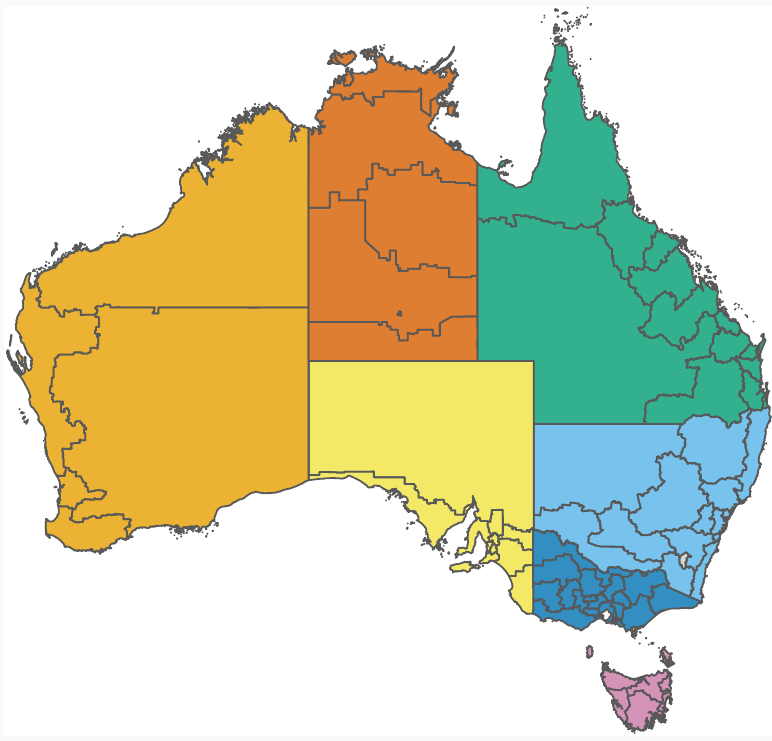
\includegraphics[width=14cm,height=7cm]{figs/aus_map_nolegend.png}}
\end{textblock}

\begin{textblock}{5}(9.4,2.4)
\begin{block}{}%\fontsize{12}{13}\sf
  \begin{itemize}\itemsep=0cm\parskip=0cm
    \item Visitor Nights 
    \item Monthly time series
    \item 1998 -- 2019
    \item \bf{77 regions}
  \end{itemize}
\end{block}
\end{textblock}
\end{frame}

\begin{frame}{Regions V Aggregate}
\phantomsection\label{regions-v-aggregate}
\includegraphics{FLAP_files/figure-beamer/unnamed-chunk-5-1.pdf}

\pause

\includegraphics{FLAP_files/figure-beamer/unnamed-chunk-6-1.pdf}
\end{frame}

\begin{frame}{FLAP Intuition}
\phantomsection\label{flap-intuition}
We have multivariate times series:

\begin{itemize}
\tightlist
\item
  which share similar patterns;
\item
  with a better signal-noise ratio in the linear combination.
\end{itemize}

\pause

\vspace{0.3cm}

\begin{alertblock}{Can we find components that:}

\begin{enumerate}
\item are easy to forecast (or easier than the original series);
\item can capture possible common signals;
\item can improve forecast of original series.
\end{enumerate}

\end{alertblock}
\end{frame}

\begin{frame}{Outline of FLAP Implementation}
\phantomsection\label{outline-of-flap-implementation}
\begin{itemize}
\tightlist
\item
  We want to forecast a multivariate series
  \(\bm{y}_t \in \mathbb{R}^m\).
\item
  Construct many linear combinations
  \(\bm{c}_t = \bm{\Phi}\bm{y}_t  \in \mathbb{R}^p\) of the multivariate
  series.
\item
  Produce univariate forecasts of all series
  \(\textcolor{blue}{\hat{\bm{y}}_{t+h}}\) and all linear combinations
  \(\textcolor{blue}{\hat{\bm{c}}_{t+h}}\).
\item
  Project forecasts onto the \(\mathbb{R}^m\) coherent subspace,
  resulting in \(\textcolor{red}{\tilde{\bm{y}}_{t+h}}\).
\end{itemize}
\end{frame}

\begin{frame}{Geometry of FLAP}
\phantomsection\label{geometry-of-flap}
\only<1>{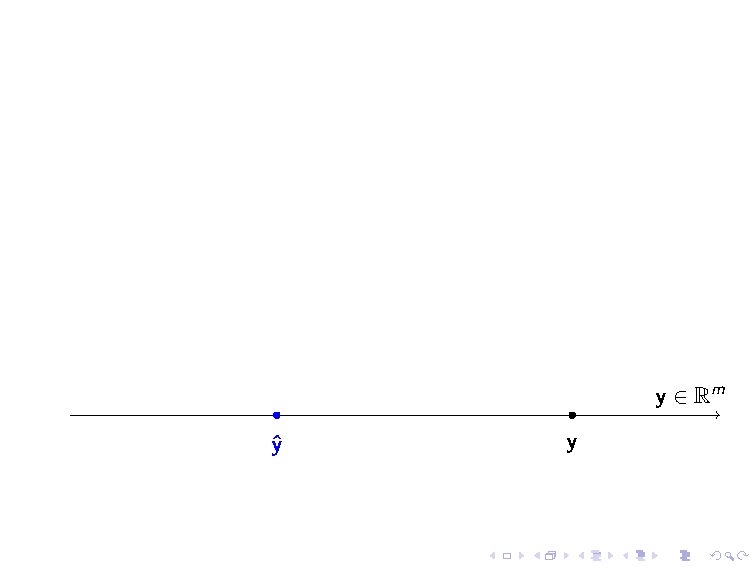
\includegraphics[page=1, width=\textwidth]{figs/FLAP_geometry.pdf}}
\only<2>{\includegraphics[page=2, width=\textwidth]{figs/FLAP_geometry.pdf}}
\only<3>{\includegraphics[page=3, width=\textwidth]{figs/FLAP_geometry.pdf}}
\only<4>{\includegraphics[page=4, width=\textwidth]{figs/FLAP_geometry.pdf}}
\only<5>{\includegraphics[page=5, width=\textwidth]{figs/FLAP_geometry.pdf}}
\end{frame}

\begin{frame}{FLAP Projection}
\phantomsection\label{flap-projection}
\vspace*{-0.6cm}

\[
\bm{z}_t = \begin{bmatrix} \bm{y}_t\\ \bm{c}_t \end{bmatrix},
\qquad \textcolor{blue}{\hat{\bm{z}}_{t+h}} = \begin{bmatrix} \textcolor{blue}{\hat{\bm{y}}_{t+h}}\\ \textcolor{blue}{\hat{\bm{c}}_{t+h}}\end{bmatrix}, 
\qquad\textcolor{red}{\tilde{\bm{z}}_{t+h}} = \bm{M} \textcolor{blue}{\hat{\bm{z}}_{t+h}}
\]

where \(\bm{M}\) is a projection matrix onto the \(\mathbb{R}^m\)
coherent subspace \vspace*{-0.4cm}

\[
\begin{aligned}
\bm{M} &= \bm{I}_{m+p} - \bm{W}_h\bm{C}'(\bm{C}\bm{W}_h\bm{C}')^{-1}\bm{C}\\
\bm{C} &= \big[- \bm{\Phi} ~~~ \bm{I}_{p}\big]\\
\bm{W}_h &= \Var(\bm{z}_{t+h} - \textcolor{blue}{\hat{\bm{z}}_{t+h}})
\end{aligned}
\] \pause

\begin{block}{}
\vspace*{-0.3cm}
$$
\textcolor{red}{\tilde{\bm{y}}_{t+h}} = 
\bm{G}\textcolor{blue}{\hat{\bm{z}}_{t+h}} = \bm{J}\bm{M}\textcolor{blue}{\hat{\bm{z}}_{t+h}}
$$\vspace*{-0.8cm}
\end{block}

\vspace*{-1cm}

\[
\bm{J} = \big[\bm{I}_m ~~~ \bm{O}_{m\times p}\big]
\]
\end{frame}

\begin{frame}{Minimum variance of individual series}
\phantomsection\label{minimum-variance-of-individual-series}
The projection is equivalent to the mapping \[
\textcolor{red}{\tilde{\bm{y}}_{t+h}} = \bm{G}\textcolor{blue}{\hat{\bm{z}}_{t+h}}~~\text{and}~~\Var(\bm{y}_{t+h} - \textcolor{red}{\tilde{\bm{y}}_{t+h}})=\bm{G}\bm{W}_h\bm{G}',
\] where
\(\bm{G} = \big[\bm{g}_1 ~~ \bm{g}_2 ~~ \dots ~~ \bm{g}_m\big]' \in \mathbb{R}^{m\times (m+p)}\)
is the solution to \[
\underset{\bm{G}}{\arg\min}\ \text{tr} (\bm{G}\bm{W}_h\bm{G}')
\qquad \text{s.t. } \bm{G}\bm{S} = \bm{I}
\] or \[
\underset{\bm{g}_i}{\arg\min}\ \bm{g}_i'\bm{W}_h\bm{g}_i
\qquad \text{s.t. } \bm{g}_i'\bm{s}_{j} = \bm{1}(i=j),
\] where
\(\bm{S} = \begin{bmatrix}\bm{I}_m \\\bm{\Phi}\end{bmatrix} = \big[\bm{s}_1\cdots \bm{s}_m\big]\).
\end{frame}

\begin{frame}{Key results}
\phantomsection\label{key-results}
\begin{enumerate}
\tightlist
\item
  The forecast error variance is \textbf{reduced} with FLAP

  \begin{itemize}
  \tightlist
  \item
    \(\Var(\bm{y}_{t+h} - \textcolor{blue}{\hat{\bm{y}}_{t+h}}) -\Var(\bm{y}_{t+h} - \textcolor{red}{\tilde{\bm{y}}_{t+h}})\)
    is \textbf{positive semi-definite}. \pause
  \end{itemize}
\end{enumerate}

\vspace*{0.3cm}

\begin{enumerate}
\setcounter{enumi}{1}
\tightlist
\item
  The forecast error variance \textbf{monotonically} decreases with
  increasing number of components

  \begin{itemize}
  \tightlist
  \item
    the diagonal elements of
    \(\Var(\bm{y}_{t+h} - \textcolor{blue}{\hat{\bm{y}}_{t+h}}) -\Var(\bm{y}_{t+h} - \textcolor{red}{\tilde{\bm{y}}_{t+h}})\)
    are non-decreasing as the number of components increases. \pause
  \end{itemize}
\end{enumerate}

\vspace*{0.3cm}

\begin{enumerate}
\setcounter{enumi}{2}
\tightlist
\item
  The forecast projection is \textbf{optimal} to achieve minimum
  forecast error variance of each series.
\end{enumerate}
\end{frame}

\begin{frame}{In practice, we need to:}
\phantomsection\label{in-practice-we-need-to}
\begin{itemize}
\tightlist
\item
  Estimate
  \(\bm{W}_h = \Var(\bm{z}_{t+h} - \textcolor{blue}{\hat{\bm{z}}_{t+h})}\).

  \begin{itemize}
  \tightlist
  \item
    Use in-sample residuals, shrink variances to their median,
    covariances to zero.
  \end{itemize}
\end{itemize}

\pause\vspace*{0.3cm}

\begin{itemize}
\tightlist
\item
  Construct the components, \(\bm{\Phi}\).

  \begin{itemize}
  \tightlist
  \item
    Principal component analysis (PCA): find the weights matrix
    \(\bm{\Phi}\) so that the resulting components
    \alert{\textbf{maximise variance}}.
  \item
    Simulation: generate values of \(\bm{\Phi}\) from a random
    distribution and normalising them to unit vectors.

    \begin{itemize}
    \tightlist
    \item
      Normal distribution
    \item
      Uniform distribution
    \item
      Orthonormal matrix
    \end{itemize}
  \end{itemize}
\end{itemize}
\end{frame}

\begin{frame}[fragile]{Simulation}
\phantomsection\label{simulation}
\begin{itemize}
\item
  Data generating process: VAR(\(3\)) with \(m=70\) variables
\item
  Innovations \(\sim N(0,\bm{I}_m)\)
\item
  Sample size: \(T=400\)
\item
  Number of repeated samples: \(220\)
\item
  Base forecasts:

  \begin{itemize}
  \tightlist
  \item
    ARIMA models using AICc (\texttt{auto.arima()} in \texttt{forecast}
    package).
  \item
    DFM structure using BIC (different model for each horizon).
  \end{itemize}
\end{itemize}
\end{frame}

\begin{frame}{Simulation}
\phantomsection\label{simulation-1}
\includegraphics{FLAP_files/figure-beamer/simulation-1.pdf}
\end{frame}

\begin{frame}[fragile]{Monthly Australian regional tourism}
\phantomsection\label{monthly-australian-regional-tourism}
\begin{itemize}
\item
  Monthly Australian tourism data by region giving 77 series, from Jan
  1998 to Dec 2019
\item
  Use expanding window time series cross-validation with \(T=84\)
  observations in first training set, and forecast horizons
  \(h=1,2,\dots,12\).
\item
  Estimate \texttt{ets()} models using the \texttt{forecast} package.
\end{itemize}
\end{frame}

\begin{frame}{Monthly Australian regional tourism}
\phantomsection\label{monthly-australian-regional-tourism-1}
\includegraphics{FLAP_files/figure-beamer/series-1.pdf}
\end{frame}

\begin{frame}{Monthly Australian regional tourism}
\phantomsection\label{monthly-australian-regional-tourism-2}
\includegraphics{FLAP_files/figure-beamer/components-1.pdf}
\end{frame}

\begin{frame}{Monthly Australian regional tourism - \texttt{ets()}}
\phantomsection\label{monthly-australian-regional-tourism---ets}
\includegraphics{FLAP_files/figure-beamer/visnights-1.pdf}
\end{frame}

\begin{frame}{FRED-MD}
\phantomsection\label{fred-md}
\begin{itemize}
\item
  Monthly data of macroeconomic variables (McCracken and Ng, 2016).
\item
  Data from Jan 1959 -- Sep 2023. 777 observations on 122 series.
\item
  Same cleaning process as per McCracken and Ng (2016).
\item
  All series scaled to have mean 0 and variance 1.
\item
  Expanding time series cross-validation with initial size of 25 years
  and forecast horizon 12 months.
\end{itemize}
\end{frame}

\begin{frame}{FRED-MD}
\phantomsection\label{fred-md-1}
\includegraphics{FLAP_files/figure-beamer/fred-md-arima-1.pdf}
\end{frame}

\begin{frame}{Future research directions}
\phantomsection\label{future-research-directions}
\begin{itemize}
\item
  Investigate why PCA performs better than random weights
\item
  Find other components that are better than PCA
\item
  Find optimal components by minimising forecast error variance with
  respect to \(\bm{\Phi}\)
\item
  Use forecast projection and forecast reconciliation together
\end{itemize}
\end{frame}

\begin{frame}[fragile]{Working Paper and R Package}
\phantomsection\label{working-paper-and-r-package}
\fontsize{10}{8}\sf

\fullcite{flap}

\fontsize{12}{8}\sf

You can install the stable version from CRAN

\begin{Shaded}
\begin{Highlighting}[]
\DocumentationTok{\#\# CRAN.R{-}project.org/package=flap}
\FunctionTok{install.packages}\NormalTok{(}\StringTok{"flap"}\NormalTok{)}
\end{Highlighting}
\end{Shaded}

or the development version from Github

\begin{Shaded}
\begin{Highlighting}[]
\DocumentationTok{\#\# github.com/FinYang/flap}
\CommentTok{\# install.packages("remotes")}
\NormalTok{remotes}\SpecialCharTok{::}\FunctionTok{install\_github}\NormalTok{(}\StringTok{"FinYang/flap"}\NormalTok{)}
\end{Highlighting}
\end{Shaded}
\end{frame}

\begin{frame}{Slides and other information}
\phantomsection\label{slides-and-other-information}
\textbf{Slides:}

\href{https://github.com/GeorgeAthana/2024-INFORMS}{\color{Blue}{https://github.com/GeorgeAthana/2024-INFORMS}}

\vspace*{1cm}

\textbf{Other information:}

\href{https://research.monash.edu/en/persons/george-athanasopoulos}{\color{Blue}{https://research.monash.edu/en/persons/george-athanasopoulos}}

\vspace*{0.5cm}

\alert{Thank you!}
\end{frame}


\begin{frame}[allowframebreaks]{}
  \bibliographytrue
  \printbibliography[heading=none]
\end{frame}



\end{document}
